\documentclass[tikz,margin=5mm]{standalone}
\usetikzlibrary{
  3d,
  spath3,
  patterns.meta,
  decorations.pathmorphing}
\begin{document}
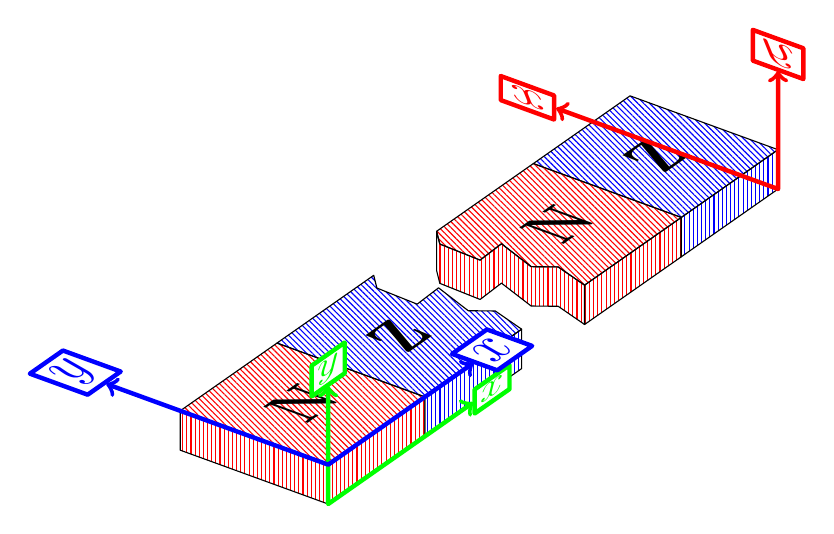
\begin{tikzpicture}[
  dec/.style={
    /utils/exec=\pgfmathsetseed{42},
    decoration={random steps,segment length=10pt,amplitude=5pt}},
  line join=round,
  % the pattern
  /pgf/pattern keys/every pattern/.style={distance=1.5pt},
  north/.style ={pattern color=red,  pattern={Lines[every pattern,angle= 90]}},
  north'/.style={pattern color=red,  pattern={Lines[every pattern,angle=-45]}},
  south/.style ={pattern color=blue, pattern={Lines[every pattern,angle= 90]}},
  south'/.style={pattern color=blue, pattern={Lines[every pattern,angle=-45]}},
  % 3d stuff
  front face/.style={canvas is yz plane at x={depthOfPiece(#1)}},
  front face/.default=0,
  side face/.style ={canvas is xz plane at y=0},
  top face/.style  ={canvas is xy plane at z=Height},
  x=(35:.75cm), y=(160:1cm), z=(90:.5cm),
  % geometry
  declare function={
    Height = 1;   % z direction
    Width  = 2;   % y direction
    Depth  = 2;   % x direction
    dDepth = 1.3; % distance between broken pieces
    depthOfPiece(\x) = % evals x value for piece's closest corner to viewer
      \x * Depth + (\x >= 2) * dDepth;}
  ]
% create the ragged line and save it
\path[dec,decorate] (0,0,0) -- (0, Width, 0) [spath/save=ragged line];

% front face
\draw[front face, north] (0,0) rectangle +(Width, Height);

% side pieces
\foreach[count=\piece from 0] \style in {north, south, north, south}
  \draw[side face, \style]
    (depthOfPiece \piece, 0) rectangle +(Depth, Height);

% top face
\begin{scope}[top face, transform shape, font=\Huge\bfseries]
  % the unbroken ones are easy
  \foreach \piece/\style/\text in {0/north'/N, 3/south'/Z}
    \draw[\style] (depthOfPiece \piece,0) rectangle
      node {\text} +(Depth, Width);
  
  % the broken ones are not
  % could be made with \foreach and a complex variable path
  \draw[south'] (depthOfPiece 1,0) -- +(right:Depth)
       [spath/append=ragged line]  -| cycle
   node at (depthOfPiece 1.5,.5*Width) {Z};
  \draw[north'] (depthOfPiece 2,0) [spath/append=ragged line]
        -- + (right:Depth) |- cycle
   node at (depthOfPiece 2.5,.5*Width) {N};
\end{scope}

% the broken front face
% this is where spath3 is necessary because the inverse is needed
\draw[front face=2, north]
  (0,0) [spath/append=ragged line] -- ++(up: Height)
        [spath/append reverse=ragged line] -- cycle;

% debug faces
\foreach \face/\col in {front/red, side/green, top/blue}
  \draw[ultra thick, transform shape, <->, \face\space face=4,
    \col, font=\Huge, nodes={fill=white, draw}]
    (0,3) node[above]{$y$} |- (3,0) node[right]{$x$};
\end{tikzpicture}

\tikz[
  dec/.style={
    /utils/exec=\pgfmathsetseed{42},
    decoration={random steps,segment length=10pt,amplitude=5pt}}]
\matrix[column sep=5mm, ultra thick, every path/.append style={fill=gray}]{
  \draw      (0,0) decorate[dec] {-- (1,0)}
    (0,0) -- (0,1) decorate[dec] {-- (1,1)} -- (1,0);
  &
  \draw[line cap=round, line join=round]
             (0,0) decorate[dec] {-- (1,0)}
    (0,0) -- (0,1) decorate[dec] {-- (1,1)} -- (1,0);\\};
\end{document}